% Created 2023-01-12 Πεμ 16:53
% Intended LaTeX compiler: pdflatex
\documentclass[11pt]{article}
\usepackage[utf8]{inputenc}
\usepackage[T1]{fontenc}
\usepackage{graphicx}
\usepackage{longtable}
\usepackage{wrapfig}
\usepackage{rotating}
\usepackage[normalem]{ulem}
\usepackage{amsmath}
\usepackage{amssymb}
\usepackage{capt-of}
\usepackage{hyperref}
\usepackage{booktabs}
\usepackage{import}
\usepackage[LGR, T1]{fontenc}
\usepackage[greek, english]{babel}
\usepackage{alphabeta}
\usepackage{esint}
\usepackage{mathtools}
\usepackage{esdiff}
\usepackage{makeidx}
\usepackage{glossaries}
\usepackage{newfloat}
\usepackage{minted}
\usepackage{chemfig}
\usepackage{svg}
\usepackage[a4paper, margin=3cm]{geometry}
\author{Βιδιάνος Γιαννίτσης}
\date{\today}
\title{Ανάλυση του block 400 - Παραγωγή Γλυκερόλης}
\hypersetup{
 pdfauthor={Βιδιάνος Γιαννίτσης},
 pdftitle={Ανάλυση του block 400 - Παραγωγή Γλυκερόλης},
 pdfkeywords={},
 pdfsubject={},
 pdfcreator={Emacs 28.2 (Org mode 9.5.5)}, 
 pdflang={English}}
\makeatletter
\newcommand{\citeprocitem}[2]{\hyper@linkstart{cite}{citeproc_bib_item_#1}#2\hyper@linkend}
\makeatother

\usepackage[notquote]{hanging}
\begin{document}

\maketitle
\tableofcontents

\renewcommand{\abstractname}{Περίληψη}
\renewcommand{\tablename}{Πίνακας}
\renewcommand{\figurename}{Σχήμα}
\renewcommand\listingscaption{Κώδικας}

\section{Διάγραμμα ροής και Επεξήγηση}
\label{sec:orgc362d2b}
\begin{figure}[htbp]
\centering
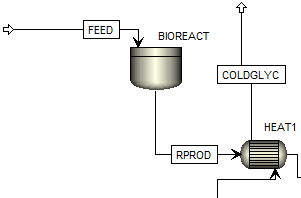
\includegraphics[width=.9\linewidth]{Διάγραμμα_ροής_και_Επεξήγηση/2023-01-12_16-53-41_screenshot.png}
\caption{Διάγραμμα ροής του block 400}
\end{figure}


Στο block 400 όπως προαναφέρθηκε γίνεται η παραγωγή της γλυκερόλης στον βιοαντιδραστήρα, του οποίου το προιόν προθερμαίνεται με το ρεύμα της καθαρής γλυκερόλης του block 500. Στο διάγραμμα ροής φαίνονται ο βιοαντιδραστήρας και ο εναλλάκτης θερμότητας που απαιτούνται.

\section{Σχεδιαστικές Επιλογές}
\label{sec:orgb921809}
Η βασική σχεδιαστική επιλογή του block αυτού είναι ο τύπος και η λειτουργία του βιοαντιδραστήρα. Για τον εναλλάκτη δεν χρειάζεται να αναφερθεί κάτι καθώς ο σκοπός του είναι βασικά να ψύξει την παραγόμενη γλυκερόλη, το οποίο μπορεί να γίνει ταυτόχρονα με την προθέρμανση του ρεύματος εξόδου του αντιδραστήρα, άρα ήταν μία εύκολη επιλογή που βοηθάει στην ενεργειακή ολοκλήρωση της διεργασίας.

Για τον αντιδραστήρα, ο τύπος που επιλέχθηκε είναι ο αντιδραστήρας RBatch. Αυτό έγινε διότι η λειτουργία διαλείποντος έργου είναι αρκετά διαδεδομένη στους βιοαντιδραστήρες για 2 βασικούς λόγους. Ο πρώτος είναι πως οι αντιδράσεις αυτές έχουν αυτοκαταλυτική φύση άρα σε μία διάταξη συνεχούς ροής, υπάρχει βιομάζα στην έξοδο του αντιδραστήρα αντί να συσσωρεύεται όλη στον αντιδραστήρα, το οποίο μειώνει τον ρυθμό αντίδρασης, ενώ ο δεύτερος είναι ότι σε μία μικροβιακή καλλιέργεια, η οποία λειτουργεί σε μόνιμες συνθήκες, υπάρχει πάντα η πιθανότητα επιμόλυνσης του αντιδραστήρα. Στις περισσότερες περιπτώσεις, η επιμόλυνση αυτή δεν θα δράσει βοηθητικά για τον μικροοργανισμό μας και θα μειώσει τον ρυθμό της αντίδρασης και πιθανότατα την καθαρότητα του προιόντος. Όταν παρατηρηθεί κάτι τέτοιο, θα πρέπει να γίνει ολικό shut down του αντιδραστήρα και να καθαριστεί, το οποίο αποτελεί ένα μεγάλο διάστημα μη παραγωγικού χρόνου μέχρι να ξαναρχίσει το σύστημα σε μόνιμη κατάσταση. Στην περίπτωση του batch αντιδραστήρα, αυτός καθαρίζεται σε κάθε batch και λειτουργεί σε μη μόνιμη κατάσταση, άρα δεν χάνεται χρόνος για την αποκατάσταση της μόνιμης κατάστασης. Επίσης, είναι σημαντικά μικρότερη η πιθανότητα επιμόλυνσης.

Επιπλέον, ένας αντιδραστήρας CSTR πρέπει να λειτουργεί σε τέτοιες συνθήκες ώστε να μην οδηγηθεί σε μόνιμη κατάσταση έκπλυσης, κάτι το ανεπιθύμητο. Αυτό σημαίνει, πως για την τροφοδοσία του αντιδραστήρα μας, ο όγκος που απαιτείται είναι τουλάχιστον 3 φορές μεγαλύτερος αυτού του batch και αυτό είναι χωρίς να ληφθεί υπόψην η αργή κινητική, λόγω της οποίας ο όγκος μπορεί να είναι ακόμη μεγαλύτερος. Θεωρητικά, αυτό θα μπορούσε να λυθεί σε έναν αντιδραστήρα PFR, όμως η ανάδευση είναι ιδιαίτερα σημαντική στις αερόβιες μικροβιακές καλλιέργειες καθώς βοηθάει στην ομοιογένεια και στην συνεχή αιώρηση της βιομάζας, παράγοντες που επιτρέπουν την γρηγορότερη ανάπτυξη της. Επίσης, βελτιώνεται η διασπορά του δυσδιάλυτου οξυγόνου το οποίο πρέπει να υπάρχει και σε ορισμένες περιπτώσεις η μεταφορά του είναι από τα πιο βραδέα στάδια της διεργασίας. Για αυτό, οι αντιδραστήρες PFR δεν προτιμούνται συνήθως για τέτοιες διεργασίες, εκτός από ορισμένες περιπτώσεις κλινών στις οποίες υπάρχει ακινητοποιημένη βιομάζα, μία διεργασία η οποία είναι ιδιαίτερα περίπλοκη στην μελέτη της.

Όλοι αυτοί είναι λόγοι για τους οποίους δεν προτιμάται ένα σύστημα συνεχούς ροής, ακόμη και στην περίπτωση που θέλουμε πολύ υψηλή παραγωγικότητα στον αντιδραστήρα.

Για τις συνθήκες λειτουργίας του, εφόσον έχουμε μία καθαρή καλλιέργεια ενός μικροοργανισμού, οι βέλτιστες συνθήκες λειτουργίας είναι αυστηρά καθορισμένες από τον μικροοργανισμό και είναι τυπικά σε ένα στενό εύρος τιμών το οποίο βρίσκεται από βιβλιογραφία. Για τον μικροοργανισμό Candida glycerinogenes ο οποίος έχει χρησιμοποιηθεί στην διεργασία αυτή, βρέθηκε βιβλιογραφικά πως η βέλτιστη συγκέντρωση γλυκόζης είναι 230-250 g/l, η συγκέντρωση ουρίας 2 g/l, η συγκέντρωση φωσφόρου 55-60 mg/l (προστίθεται στην μορφή του corn steep liquor με βάση την βιβλιογραφία), το pH μεταξύ 4-6 και η θερμοκρασία μεταξύ 29 και 33 \(^oC\) \textsuperscript{\citeprocitem{1}{1}} . Για τα θρεπτικά συστατικά, βρέθηκε η ποσότητα νερού που απαιτείται για την παραγωγή διαλύματος γλυκόζης 230 g/l με όλη την γλυκόζη της διεργασίας και έπειτα η ποσότητα ουρίας και corn steep liquor (CSL) που απαιτείται ώστε οι συγκεντρώσεις τους να είναι οι επιθυμητές. Το pH δεν χρειάζεται να ρυθμιστεί σε κάποιο επίπεδο καθώς παρουσία του CSL το pH είναι στην επιθυμητή περιοχή ενώ η θερμοκρασία ρυθμίστηκε στους 30 \(^oC\) καθώς για αυτή την τιμή υπάρχουν κινητικά δεδομένα \textsuperscript{\citeprocitem{2}{2}} . Το CSL δεν προστέθηκε στην προσομοίωση της διεργασίας καθώς δεν υπάρχει στην βάση δεδομένων του Aspen και η πολυπλοκότητα της διεργασίας θα αυξανόταν σημαντικά με την προσθήκη του.

\section{Υπολογισμοί}
\label{sec:org592712b}
Οι βασικοί υπολογισμοί του block 400 είναι 3. Η στοιχειομετρία της μικροβιακής αντίδρασης, η οποία δεν είναι γνωστή εξ'αρχής, η κινητική της μικροβιακής αντίδρασης και οι υπολογισμοί του εναλλάκτη. Οι υπολογισμοί του εναλλάκτη έγιναν απευθείας στο Aspen για αυτό θα επεξηγηθούν περισσότερο στην προσομοίωση. Για την στοιχειομετρία και την κινητική της μικροβιακής αντίδρασης, βασιστήκαμε σε πειραματικά δεδομένα \textsuperscript{\citeprocitem{1}{1},\citeprocitem{2}{2}} . Ο προσδιορισμός της στοιχειομετρίας της αντίδρασης είναι μία περίπλοκη διαδικασία, ειδικά επειδή δεν είναι γνωστός εκ των προτέρων ο τύπος της βιομάζας. Υπάρχουν διάφορες τεχνικές που μπορούν να ακολουθηθούν για τον προσδιορισμό αυτόν, αλλά αποφασίστηκε πως αντί να υποτεθεί ο μοριακός τύπος της βιομάζας και να προκύψει μία αυθαίρετη μικροβιακή αντίδραση, να υπολογιστούν όσοι συντελεστές μπορούν με βάση τα πειραματικά δεδομένα για τα yields της αντίδρασης και να υπολογιστούν από αυτά ο τύπος της βιομάζας και όσοι στοιχειομετρικοί συντελεστές δεν είναι πειραματικά γνωστοί. Η αναλυτική επεξήγηση των υπολογισμών αυτών παρατίθεται σε σχετικό παράρτημα. Προκύπτει πως η αντίδραση είναι η

\[ 1.22 S + 0.24U + 2.89 O_2 \rightarrow 0.45 C_{1.48}H_{2.95}O_{0.048}N_{0.11} + G + 0.025E + 0.019Ac + 3.5CO_2 + 2.5H_2O \]
όπου S η γλυκόζη (υπόστρωμα), U η ουρία, G η γλυκερόλη, Ε η αιθανόλη και Ac το οξικό οξύ.

Για την κινητική της μικροβιακής αντίδρασης, έγινε προσαρμογή των παραπάνω πειραματικών δεδομένων στο μοντέλο Monod, το οποίο είναι το πιό κλασσικό μοντέλο για την μικροβιακή ανάπτυξη. Το πραγματικό κινητικό μοντέλο ενδέχεται να είναι πιό περίπλοκο από αυτό, αλλά απουσία μίας ολοκληρωμένης κινητικής μελέτης, το μοντέλο Monod είναι μία καλή πρώτη προσέγγιση. Ο ρυθμός με βάση το μοντέλο Monod είναι ο ρυθμός ανάπτυξης της βιομάζας. Με βάση την στοιχειομετρία όμως, ο ρυθμός της αντίδρασης ο οποίος θα χρησιμοποιηθεί στην διαστασιολόγηση του αντιδραστήρα θα είναι ο \(\frac{1}{0.45} \frac{dx}{dt}\).

Με βάση τα δεδομένα αυτά, το κινητικό μοντέλο που προέκυψε είναι το εξής:
\[ \frac{dx}{dt} = \frac{3.06*10^{-6}[S]}{236.19+[S]}[x] \] όπου οι σταθερές μ\textsubscript{max} και K\textsubscript{s} είναι υπολογισμένες σε μονάδες SI και οι συγκεντρώσεις σε g/l. Η προσαρμογή έγινε μέσω του Excel, το οποίο αρχείο μπορεί να βρεθεί \href{https://github.com/Vidianos-Giannitsis/Process-Design/blob/master/Calculations/c\_glycerinogenes\_kinetics.ods}{εδώ}.

\section{Προσομοιώσεις στο Aspen}
\label{sec:org60f2c86}
Το ρεύμα εισόδου της διεργασίας ορίστηκε με βάση τις συγκεντρώσεις που αναφέρθηκαν παραπάνω ως βέλτιστες. Έπειτα, ορίστηκε νερό ως ο διαλύτης σε μία ποσότητα τέτοια ώστε να υπάρχει όση γλυκόζη στο ρεύμα όση πρέπει να υπάρχει με βάση το block 200. Για τον βιοαντιδραστήρα, ορίστηκε ότι θα λειτουργεί σε σταθερή πίεση και θερμοκρασία (30 \(^oC\), 1 bar), με χρόνο λειτουργίας 80 ώρες (ο χρόνος που υπήρχε στα πειραματικά δεδομένα).

Για την κινητική, ορίστηκε η παραπάνω στοιχειομετρία, ενώ για την προσομοίωση του μοντέλου Monod, μπορεί να χρησιμοποιηθεί το μοντέλο LHHW με k=1, E=0, driving force τον αριθμητή του μοντέλου Monod και adsorption των παρανομαστή του. Αξίζει να αναφερθεί πως πρέπει οι μονάδες να είναι σε SI (όπως είναι στην προκειμένη περίπτωση) και στο Aspen πρέπει να μπούν οι λογάριθμοι των σταθερών και όχι οι ίδιες οι σταθερές. Επίσης, πρέπει να επιλεγεί το [C\textsubscript{i}] basis στο μενού του driving force ως mass concentration για να έχουν οι συγκεντρώσεις τις σωστές μονάδες.

Για τον εναλλάκτη του block, πρακτικά μας ενδιαφέρει να ψύξουμε το ρεύμα της καθαρής γλυκερόλης καθώς έτσι και αλλιώς δεν θα επαρκέσει για να φτάσει το ρεύμα την επιθυμητή θερμοκρασία. Για αυτό ψάχνουμε την χαμηλότερη θερμοκρασία που μπορούμε να πάμε το ρεύμα, η οποία προκύπτει πως είναι 44 \(^oC\), δηλαδή ένα ΔΤ = 14 \(^oC\) από την είσοδο του ψυχρού. Τα προιόντα του αντιδραστήρα είναι σε αρκετά μεγαλύτερη παροχή από ότι το ρεύμα αυτό, για αυτό στην αρχή του block 500 ολοκληρώνεται η θέρμανση αυτή.

\section{Βιβλιογραφία}
\label{sec:org6cefe02}
\hypertarget{citeproc_bib_item_1}{(1) Zhuge, J.; Fang, H.-Y.; Wang, Z.-X.; Chen, D.-Z.; Jin, H.-R.; Gu, H.-L. Glycerol Production by a Novel Osmotolerant Yeast Candida Glycerinogenes. \textit{Applied microbiology and biotechnology} \textbf{2001}, \textit{55} (6), 686–692. \url{https://doi.org/10.1007/s002530100596}.}

\hypertarget{citeproc_bib_item_2}{(2) Jin, H.; Fang, H.; Zhuge, J. By-Product Formation by a Novel Glycerol-Producing Yeast, Candida Glycerinogenes, with Different O2 Supplies. \textit{Biotechnology letters} \textbf{2003}, \textit{25} (4), 311–314. \url{https://doi.org/10.1023/A:1022349401575}.}
\end{document}